\section{pca2densityfile} \label{sec-pca2densityfile}

\subsection{General}

The \emph{pca2densityfile} functions similar to the
\emph{pca2densitymap} tool outlined in section
\ref{sec-pca2densitymap}. It generates a two dimensional histogram
across a 2 dimensional PCA projection by selection of a grid
spacing. The tool then writes the densities for each tile to a text
file that can be used for further processing, or external
visualization tools.

\subsection{Usage}

The \emph{pca2densityfile} tool can be called like:
\lstset{language=bash,
  caption={Calling the \emph{pca2densityfile} tool},
  label=lst-pca2densityfile-call}
\begin{lstlisting}
pca2densityfile [fasta] [pca] [dimensions] [interval-length] > [densityfile]
\end{lstlisting}
with the arguments:
\begin{enumerate}
  \item \emph{fasta} A FASTA file that has been transformed to a k-mer
    representation (i.e. using \emph{fasta2kmer} as shown in section
    \ref{sec-fasta2kmer}) and where such a k-mer representation has been
    projected onto a PCA subspace (i.e. using \emph{kmer2pca} as
    outlined in section \ref{sec-kmer2pca}.)
  \item \emph{pca} The projections onto the principal components.
  \item \emph{dimensions} How many principal components have been
    retained, the dimensionality of the PCA subspace stored in the
    \emph{pca} file.
  \item \emph{interval-length} The grid distance, i.e. the tile size
    of the histogram.
  \item \emph{densityfile} A text file where for each tile a density
    value is stored.
\end{enumerate}

\subsection{Example}
\lstset{language=bash,
  caption={Example of the \emph{pca2densityfile} tool},
  label=lst-pca2densityfile-example}
\begin{lstlisting}
pca2densitymap test.fasta test.pca 7 0.1 > /tmp/out
\end{lstlisting}
In this example a dataset of sequences \emph{test.fasta} and a
representation in a 7 dimensional PCA subspace obtained from a k-mer
representation of the sequences \emph{test.pca} is examined. A
histogram is generated using a grid spacing (tile size) of 0.1
[k-mer frequencies]. The number of sequences per tile is
printed to the output file \emph{/tmp/out}.
\lstset{language={},
  caption={Example output of the \emph{pca2densityfile} tool},
  label=lst-pca2densityfile-output}
\begin{lstlisting}
   shift x:  8.45373440
   shift y:  5.56738997
n points x:    122
n points y:     89
0 0 0
1 0 0
2 0 0
3 0 0
4 0 0
5 0 0
6 0 0
7 0 0
8 0 0
9 0 0
10 0 0
11 0 0
12 0 0
13 0 0
14 0 0
15 0 0
\end{lstlisting}
In the beginning of the output file a shift x and y value
which tells us about the origin of the file is found. Further the file shows us
how many tiles were generated according to the \emph{interval-length}
parameter. This header is followed by the data which is represented as
three values per line.
Following the header the data is represented as follows:
On each line the x and y coordinate ( of the tile ) i.e. the
number of tile that you are in, and the number of sequences present in this
square are shown. Such a file can be used with
3rd party visualization tools, such as Blender \cite{blender} in
order to inspect the density of sequences in three dimensions. An
example is shown in figure \ref{fig-pca2densityfile}.
\begin{figure}
  \begin{center}
    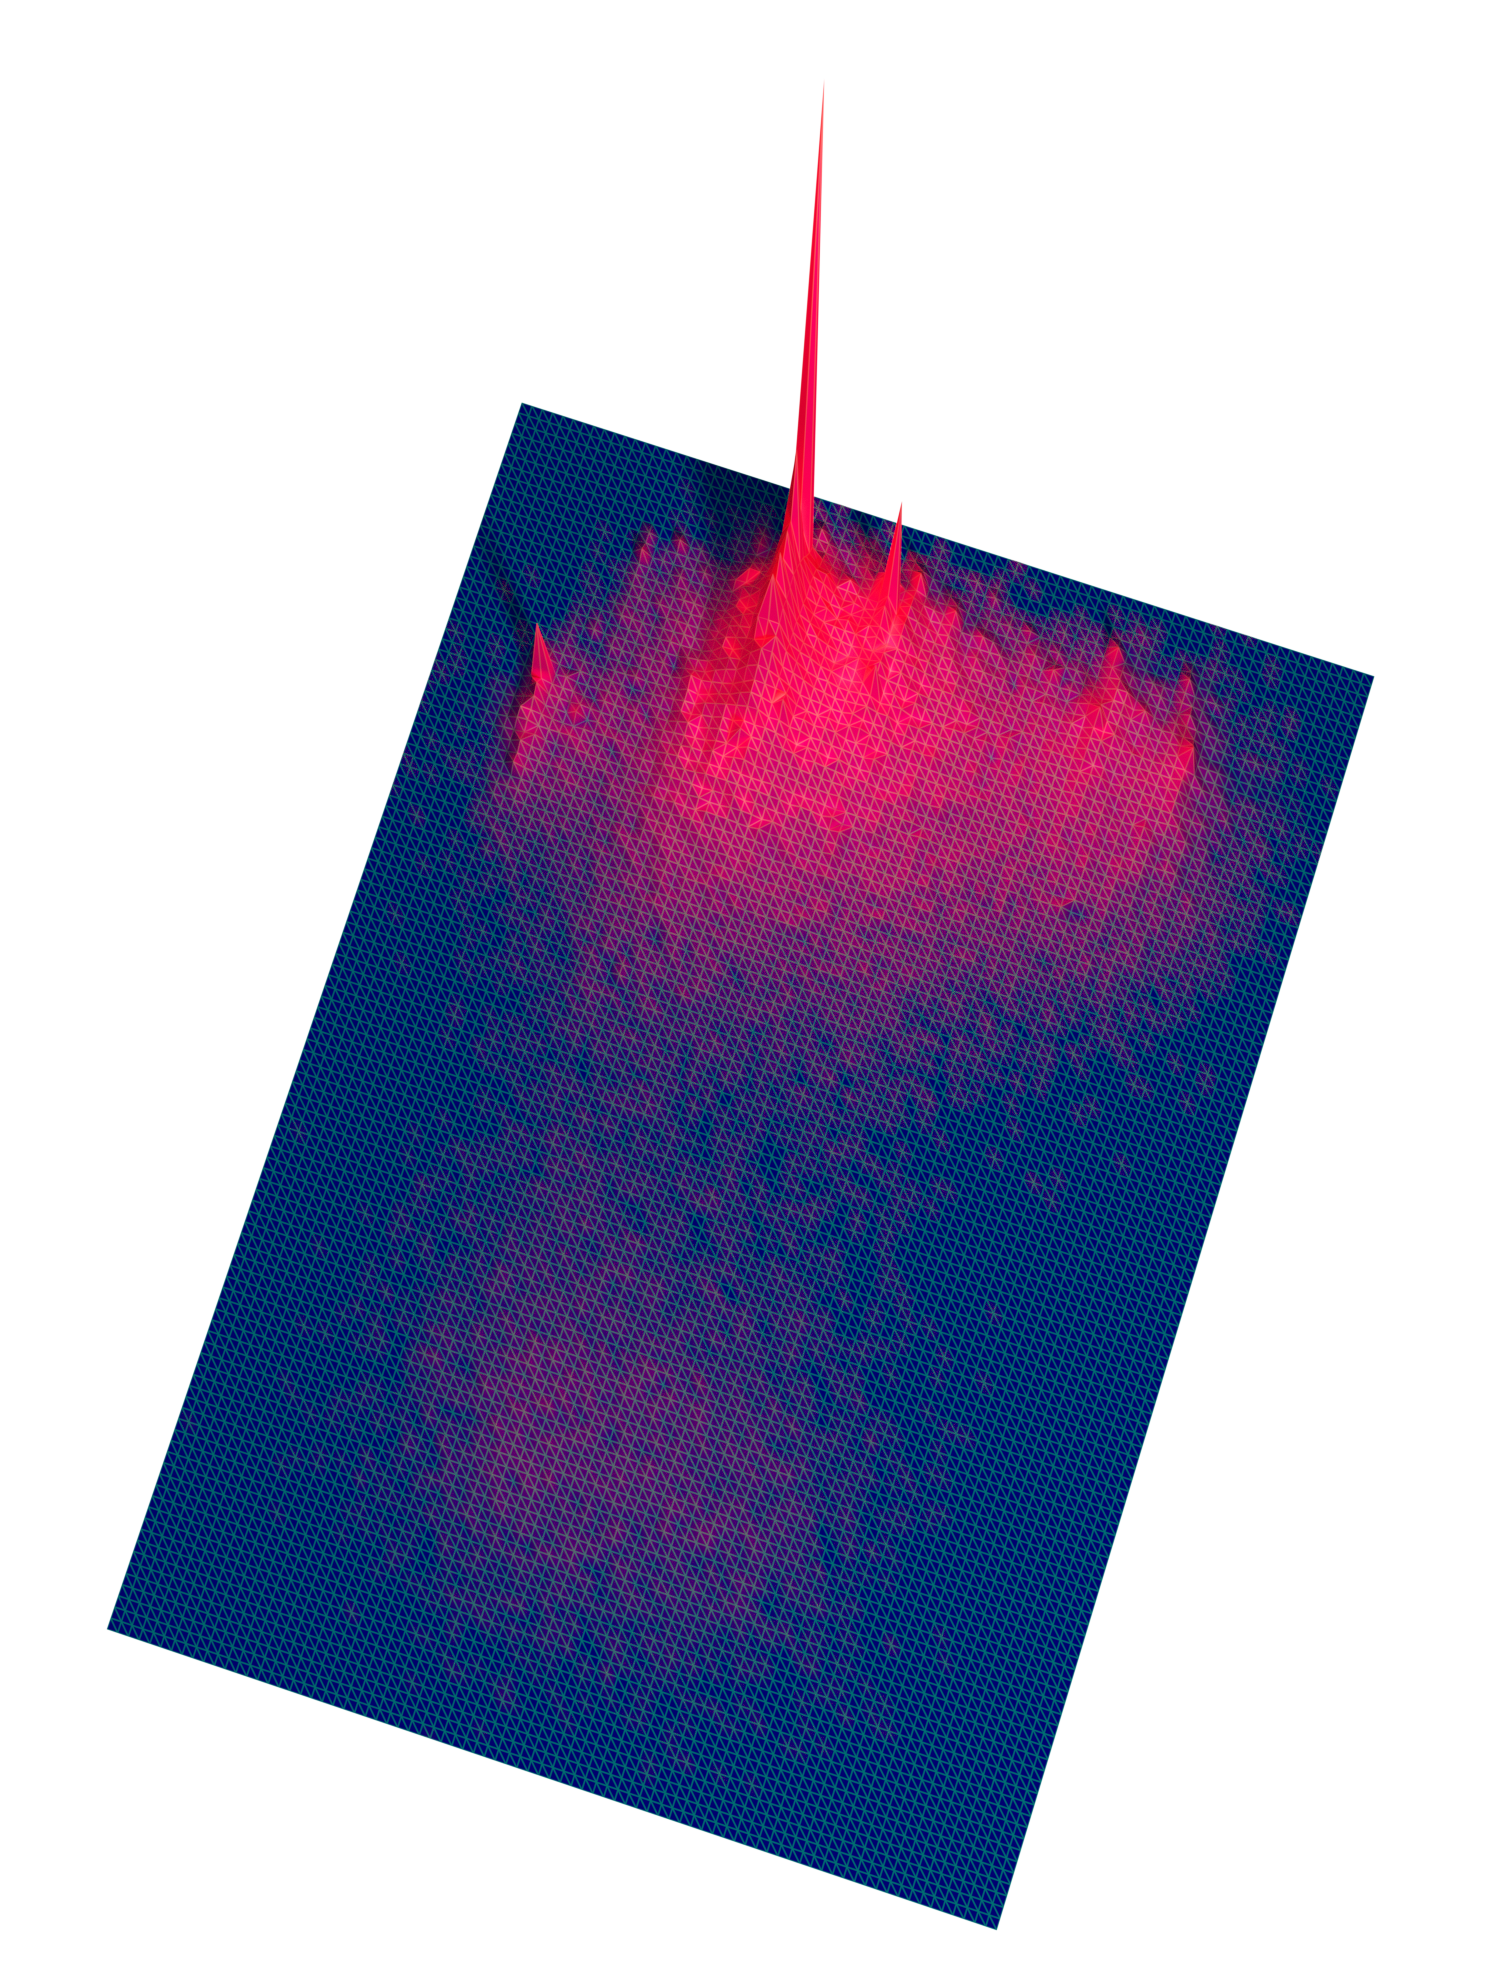
\includegraphics{pca-density-file.png}
    \caption{The output of \emph{pca2densityfile} visualized with
      Blender \cite{blender}}
    \label{fig-pca2densityfile}
  \end{center}
\end{figure}
We also provide a Blender import script for Blender 2.80 and 2.90
in the following:
\lstset{language=python,
  caption={Python script to import the output of the \emph{pca2densityfile} tool into Blender.},
  label=lst-pca2densityfile-blender}
\begin{lstlisting}
import bpy

def add_map_from_density_file(filename, objname, delta, scalefactor):
    f = open(filename, "r")

    line = f.readline();
    line_array = line.split();
    shift_x = float(line_array[2]);

    line = f.readline();
    line_array = line.split();
    shift_y = float(line_array[2]);

    line = f.readline();
    line_array = line.split();
    n_points_x = int(line_array[3]);

    line = f.readline();
    line_array = line.split();
    n_points_y = int(line_array[3]);

    verticies = [];
    faces = [];

    n_points = n_points_x*n_points_y

    for i in range(n_points):
        line = f.readline()
        line_array = line.split();
        current_point = [(delta*float(line_array[0])-shift_x,
                          delta*float(line_array[1])-shift_y,
                          float(line_array[2])*scalefactor)]
        verticies.extend(current_point)

    for j in range(n_points_y-1):
        for i in range(n_points_x-1):
            current_face = [(j*n_points_x+i,(j+1)*n_points_x+i,
                            (j+1)*n_points_x+i+1,j*n_points_x+i+1)]
            faces.extend(current_face)

    themesh = bpy.data.meshes.new(objname)
    theobject = bpy.data.objects.new(objname, themesh)
    
    bpy.data.objects.new(objname, themesh)
    bpy.context.scene.collection.objects.link(theobject)

    themesh.from_pydata(verticies, [], faces)
    themesh.update(calc_edges=True)

    return theobject

rescale = 5.;

add_map_from_density_file("/tmp/desityfile", "surface-name", 0.1, 0.03/rescale)
\end{lstlisting}
where you have to adapt \emph{/tmp/densityfile} to the location of your
output, \emph{surface-name} to the name that you want to attribute to your 3D
surface, \emph{0.1} to the grid spacing that you have chosen and
\emph{0.03} to your rescale factor.

\subsection{Implementation}
The interface to this tool is implemented in \emph{pca2denistyfile.c}.
The inner workings are implemented in \emph{density.c}.

